\documentclass[conference]{IEEEtran}
\IEEEoverridecommandlockouts
% The preceding line is only needed to identify funding in the first footnote. If that is unneeded, please comment it out.
\usepackage{cite}
\usepackage{amsmath,amssymb,amsfonts}
\usepackage{algorithmic}
\usepackage{graphicx}
\usepackage{textcomp}
\usepackage{xcolor}
\usepackage{tikz}
\usepackage{verbatim} 

\usetikzlibrary{positioning}
\def\BibTeX{{\rm B\kern-.05em{\sc i\kern-.025em b}\kern-.08em
    T\kern-.1667em\lower.7ex\hbox{E}\kern-.125emX}}
\begin{document}

\title{Machine Learning Autoencoder Applied to Communication Channels}


\author{\IEEEauthorblockN{Eduardo Dadalto Camara Gomes}
\IEEEauthorblockA{\textit{Department of Electronics, Optronics and Signal Processing (DEOS) } \\
\textit{ISAE-SUPAERO}\\
Toulouse, France \\
Email: edadaltocg@gmail.com}}


\maketitle

\begin{abstract}

write in the end.

\end{abstract}

\begin{IEEEkeywords}
communication system, machine learning, autoencoder,channel decoding, maximum a posteriori (MAP) decoder 
\end{IEEEkeywords}

\section{Introduction}
\subsection{Motivation}
Communication systems are widely present in  everyday life and have different structures. These designs are less or more complex; nevertheless, they share a common core. The simpler real communication architecture defines the system as an exchange of information between two terminals through a noisy channel. As a result of imperfections, Shannon theorized \cite{b1} in 1948 the ultimate reliable data rate that can be transmitted through a communication systems of this kind. 

Since then, the research community in digital communication developed a series of algorithms to minimize bit error rate (BER) over a channel. However, the challenge of finding an \textit{efficient} solution  (i.e., at same time low latency and with low error probability) for low signal to noise ratio (SNR) channels, remains. Based on this vision, Tim O'Shea and Jakob Hoydis \cite{b2} pertinently noted that traditional algorithms in the field have foundations in probability theory (e.g. maximum a posteriori (MAP) estimation used as a channel decoder), hence they are usually built on top of mathematically convenient models. Often, these models does not account for all the real system's imperfections, what leads to intrinsic errors in practice, even though they are theoretically optimal error corrector machines. 

Accordingly, machine learning (ML) algorithms does not require rigidly designed models and can take effortlessly account for non-linearities. These characteristics suits them well for being used as bit error correctors. Moreover, with ML based channel encoder and channel decoder, the design of communication systems as independently working blocks becomes obsolete, as a deep neural network (DNN) is able to actuate in an end-to-end optimization of the system. As a result, an optimized autoencoder with a stochastic layer that models channel's imperfections can substitute the block based representation. Therefore, ML based communication systems could be a better representation of realistic systems and could optimize information transmission of different blocklengths and with low decoding latency, resulting ultimately in gain of bandwidth over standard methods. 

Low latency and high bandwidth wireless communication are key to critical systems, such as airplanes, satellites, cellular communication and 5G operations. The latter was studied by F. D. Calabrese et al. in \cite{b3} which  demonstrated that individual based radio resource management (RRM) algorithms were outperformed by a general learning framework, resulting in significant expense reductions, while increasing performance of a network. Thereby, ML algorithms are cardinal for future state of the art communication applications.
  
\subsection{Related work}

Recently, a significant amount of work in radio communication theory has emerged, introducing ML elements to the communication system. O'Shea et al. in \cite{osheaautoencoder} developed a channel autoencoder with optimized impairment and regularization layers to emulate channel impairments. They studied this architecture over a BSC and other channels, founding ``some promising initial capacity" for this schema. In their research, results in terms of BER over SNR of a DNN based autoencoder and a convolutional neural network (CNN) based autoencoder were treated. They used a range of SNR from $-10\text{dB}$ to $15\text{dB}$ with QPSK and QAM16 theoretical capacity as benchmarks. This analysis was conducted for a binary input message.

    
T. Gruber et. al. in a 2017 paper \cite{2018} proved that a deep learning-based channel decoder could actually learn a decoding algorithm rather than just being a simple classifier. They introduced codewords that were not been used in the training set, and the trained NN was able to correctly decode it. They also observed that structured codes are easier to learn than unstructured ones. NN for structured codes are able to generalize to the full codebook even if they have not seen all the training examples. They trained the NN for very short blocklengths ($N \leq 64$) in order to compare with MAP decoding performance.


\subsection{Problem statement}

This research will implement a ML autoencoder for BSC that outperforms the MAP decoder for a range of SNR. In its most simple form, a channel autoencoder includes an encoder, a noisy channel and an decoder. Using state-of-the art DNN algorithms to find the best solution of the problem, this work hopes to contribe to set up a higher standard in terms of performance in bit-error correction and reduced delay for digital communication applications. In a near future, this disruptive methodology for error correction using ML could replace mathematically optimal decoders which are the current guideline.


%\subsection{Notation}
%Special notations used throughout the paper

\section{Theoretical Background}


\subsection{Maximum a posteriori decoder}


The concept of a MAP decoder or Bahl-Cocke-Jelinek-Raviv (BCJR) algorithm is choosing a message which maximizes the MAP probability of the corrupted information received  by the decoder \cite{b4}. This algorithm is known for its optimality in error correction for white noise interference. MAP decoding algorithms and it's variants: Log-MAP and Max-Log-MAP, are widely used as decoders for turbo codes \cite{b7}. 

The MAP decoder is practically nonviable to implement \cite{b6}. Thus, for the purpose of implementation, its variants cited in the paragraph above are better suited. The Log-MAP is an optimal decoder, having equivalent performance to the MAP decoder. The Max-Log-MAP is a suboptimal decoder and will not be treated in this paper. Refer to \cite{b6} for specific details in the derivation of the Log-MAP algorithm.

Turbo decoding using Log-MAP decoder for an additive white Gaussian noise (AWGN) channel and for a binary symmetric channel (BSC) was studied in \cite{b5}. They analyzed the BER for small SNR and concluded that the results are sensible to SNR estimation of the real channel, since the estimation of this parameter is required for the metric calculation of the algorithm \cite{b6}. It means that if the real SNR is smaller, the decoder will not perform well. Hence, for channel characteristics that change over time, the application of a MAP algorithm is debatable. This conclusion serve as motivation for ML autoencoders, which could adapt to different SNR conditions, outperforming the MAP decoder for realistic applications.

\subsection{Neural network basics}

\tikzset{%
  every neuron/.style={
    circle,
    draw,
    minimum size=0.666cm
  },
  neuron missing/.style={
    draw=none, 
    scale=2,
    text height=0.333cm,
    execute at begin node=\color{black}$\vdots$
  },
}

\begin{figure}[!hbp]
\centering

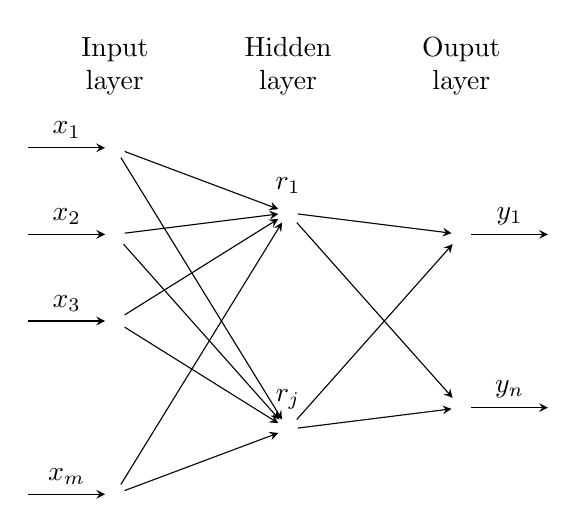
\begin{tikzpicture}[x=1.1cm, y=1.1cm, >=stealth]

\foreach \m/\l [count=\y] in {1,2,3,missing,4}
  \node [every neuron/.try, neuron \m/.try] (input-\m) at (0,2.5-\y) {};

\foreach \m [count=\y] in {1,missing,2}
  \node [every neuron/.try, neuron \m/.try ] (hidden-\m) at (2,2-\y*1.25) {};

\foreach \m [count=\y] in {1,missing,2}
  \node [every neuron/.try, neuron \m/.try ] (output-\m) at (4,1.5-\y) {};

\foreach \l [count=\i] in {1,2,3,m}
  \draw [<-] (input-\i) -- ++(-1,0)
    node [above, midway] {$x_\l$};

\foreach \l [count=\i] in {1,j}
  \node [above] at (hidden-\i.north) {$r_\l$};

\foreach \l [count=\i] in {1,n}
  \draw [->] (output-\i) -- ++(1,0)
    node [above, midway] {$y_\l$};

\foreach \i in {1,...,4}
  \foreach \j in {1,...,2}
    \draw [->] (input-\i) -- (hidden-\j);

\foreach \i in {1,...,2}
  \foreach \j in {1,...,2}
    \draw [->] (hidden-\i) -- (output-\j);

\foreach \l [count=\x from 0] in {Input, Hidden, Ouput}
  \node [align=center, above] at (\x*2,2) {\l \\ layer};

\end{tikzpicture}

\caption{MLNN representative diagram. Where \textbf{x} is the input vector of the NN, $\textbf{r}_{l}$ is a hidden layer vector
and \textbf{y} is the output vector.} \label{fig:NN}
\end{figure}

Neural networks (NN) are a set of connected \textit{neurons} able to approximate any kind of function through an architecture composed of several single processing units (neurons) connected together forming a network. They are defined by \cite{b9} as parallel distributed, learning- and self-organizing information processing systems. 

In the context of learning algorithms implemented by a NN, the key issue is to find a suitable architecture that delivers the best results. To define and build this infrastructure, the activation function, the loss function and the structure must be decided.  M. Nielson \cite{b8} in his book explores a vast amount of NN architectures and how they work. 

Multi-layer feed forward neural network (MLNN) as shown in Fig. \ref{fig:NN} will be applied in this work. They are known for the universal approximation property \cite{b9} and for the versatility of increasing the number of layers, creating a DNN able to undertake complex classification problems with low classification error and low dimensionality. In more general terms, a MLNN with $L$ layers, also called \textit{depth}, and parameter $\theta$ is a mapping of an input $\textbf{r}_0 \in \mathbb{R}^{N_0}$ to an output $\textbf{r}_L \in \mathbb{R}^{N_L}$ through $L$ iterative steps. For a fully-connected network, each layer vector is calculated in an iterative forward propagation, where each neuron is composed of a linear combinator and an activation function defined as 

\begin{equation}\label{eq:eqFP}
	f_{l}\left( \textbf{r}_{l-1};\theta _{l}\right) = \sigma \left( \textbf{W}_{l}\textbf{r}_{l-1}+\textbf{b}_{l}\right)
\end{equation}
where $\textbf{W}_{l}\in \mathbb{R} ^{N_{l}\times N_{l-1}}$ is the weight matrix between layers $l-1$ and $l$,  $\textbf{b}_{l}\in \mathbb{R} ^{N_l}$ is the bias vector and $\sigma$ is the activation function \cite{b2}.

In order to accurately classify an input, a \textit{perceptron} processing unit is chosen to solve a classification problem for each input message. A perceptron maps a binary vector input into a single binary output digit \cite{b8}. Mathematically, it means that the function defined in \eqref{eq:eqFP}, outputs $1$ or $0$, depending on a threshold value.

For a classification problem in communication, the \textit{categorical cross-entropy} loss function $l(\textbf{p},\textbf{q}):\mathbb{R} ^{N_L}\times \mathbb{R} ^{N_L}\mapsto \mathbb{R}$ defined in \eqref{eq:c-e} is most common. It is derived from the log-likelihood of a training set where $q_j$ is the estimated probability of the outcome $j$ and $p_{j}$ is the true probability. Basically, the function measures the dissimilarity between $p_{j}$ (what you expected) and $q_{j}$ (what you obtained) \cite{b10} where $j=1,...,N_L$.
\begin{equation}\label{eq:c-e}
	l(\textbf{p},\textbf{q})=-\sum _{j}p_{j}\log \left( q_{j}\right)
\end{equation}

With all these elements set, training the neural network to calculate an accurate weight matrix $\textbf{W}$ for forward propagation requires a labeled \textit{training data set}. This set is composed of pairs $ (\textbf{r}_{0,i}, \textbf{p}_i) $, where $i=1,...,S$ and $S$ is the number of training sets. It matches the input and its respective desired output. The objective is to minimize the overall loss function defined in \eqref{eq:o-c-e} in terms of the parameter $\theta$ \cite{b2}. 
\begin{equation}\label{eq:o-c-e}
L\left( \theta \right) =\dfrac {1}{S}\sum ^{S}_{i=1}l\left( \textbf{p}_{L,i},\textbf{r}_{L,i}\right)	
\end{equation}  

This problem is an optimization problem and can be solved through different algorithms. For NN, an efficient way of computing this minimization is implementing the back-propagation (BP) algorithm. 	BP is classified as a supervised learning algorithm that is able to optimize a function based on some parameter and is highly parallelizable in computational terms \cite{b8}\cite{b9}.

The great advantage of NN is its ability do generalize the training set, delivering the right results even for data not contained in the training set. With the weight matrix trained, the NN find the correct putputs for unseen inputs . In order to validate this principle, a \textit{validation data set} is used and the loss is mesured. Based on this value, we can evaluate the NN overall accuracy.

For implementing all the algorithms, Keras, a high-level python API for ML, will be used together with TensorFlow 1.13.1, a ML python friendly open-source library \cite{b11} \cite{b12}. Both are available for free.




\subsection{Autoencoders}
TO PARAPHRASE: The parallel computing
capabilities of NNs allow us to solve or, at least, approximate
the MLD problem in polynomial time [7]. Moreover, the
weights of the NN are precomputed during training and the
decoding step itself is then relatively simple. 

NNs which can learn an appropriate
mapping between noisy input patterns and codewords. No
assumption has to be made about the statistics of the channel
noise because the NN is able to learn the mapping or to
extract the channel statistics during the learning process

decoding problems have far more possibilities than conventional pattern recognition problems

In 2006, a new training technique, called layer-by-layer
unsupervised pre-training followed by gradient descent finetuning [14], led to the renaissance of NNs because it made
training of NNs with more layers feasible.

new hardware such as graphical processing units (GPUs) are available
to speed up learning as well as inference. In this renaissance
of NNs, new NND ideas emerge

The curse of dimensionality

%\section{Procedure and methods}
%Explain what I Should do to achieve my goal
\begin{comment}

\subsection{Figures and Tables}


\begin{table}[htbp]
\caption{Table Type Styles}
\begin{center}
\begin{tabular}{|c|c|c|c|}
\hline
\textbf{Table}&\multicolumn{3}{|c|}{\textbf{Table Column Head}} \\
\cline{2-4} 
\textbf{Head} & \textbf{\textit{Table column subhead}}& \textbf{\textit{Subhead}}& \textbf{\textit{Subhead}} \\
\hline
copy& More table copy$^{\mathrm{a}}$& &  \\
\hline
\multicolumn{4}{l}{$^{\mathrm{a}}$Sample of a Table footnote.}
\end{tabular}
\label{tab1}
\end{center}
\end{table}


\begin{figure}[htbp]
\centerline{\includegraphics{fig1.png}}
\caption{Example of a figure caption.}
\label{fig}
\end{figure}
\end{comment}


\begin{thebibliography}{00}
\bibitem{b1} C. E. Shannon, ``A mathematical theory of communication," Bell System Technical Journal, vol. 27, no. 3, pp. 379–423, Jul. 1948.

\bibitem{b2} O'Shea, Tim \& Hoydis, Jakob, ``An Introduction to Machine Learning Communications Systems", 2017.
\bibitem{b3} F. D. Calabrese, L. Wang, E. Ghadimi, G. Peters, and P. Soldati, ``Learning radio resource management in 5G networks: Framework,
opportunities and challenges," arXiv preprint arXiv:1611.10253, 2016
\bibitem{b4} W. Alexander, H. Peter \& W. Norbert, ``Turbo-Decoding Without SNR Estimation",IEEE Communications Letter, vol. 4, no. 6, pp. 193-195, 2000.
\bibitem{b5} M. Jordan and R. Nichols, “The effects of channel characteristics on turbo code performance,” in Proc. Milcom’96, McLean, VA, Oct. 1996, pp. 17–21.
\bibitem{b6} Robertson, P. , Hoeher, P. and Villebrun, E. (1997), Optimal and sub‐optimal maximum a posteriori algorithms suitable for turbo decoding. Eur. Trans. Telecomm., 8: 119-125. doi:10.1002/ett.4460080202.
\bibitem{b7} J. Hagenauer,P. Robertson, L. Papke: iterative (“Turbo”) decoding of systematic convolutional codes with the MAP and SOVA
algorithms. In: ITG-Fachbericht 130. October 1994, p. 21-29.
\bibitem{b8} M. Nielsen, \textit{Neural Networks and Deep Learning}.
\bibitem{b9} I. Mohamed, ``Applications of neural networks to digital communications - a survey", 1997.
\bibitem{b10} M. Kevin, ``Machine Learning: A Probabilistic Perspective", MIT, ISBN 978-0262018029, 2012.
\bibitem{b11} M. Abadi, A. Agarwal, P. Barham, et al., 
``TensorFlow: Large-scale machine learning on heterogeneous systems", 2015. Software available from tensorflow.org.
\bibitem{b12} F. Chollet, “keras,” https://github.com/fchollet/keras, 2015.
\bibitem{osheaautoencoder} T. O'Shea, K. arra, T. C. Clancy, ``Learning to Communicate: Channel Auto-encoders, Domain Specific Regularizers, and Attention", 2016.
\bibitem{2018} T. Gruber, S. Cammerer, J. Hoydis, and S. ten Brink, “On deep learning based channel decoding,” accepted for CISS 2017, arXiv preprint arXiv:1701.07738, 2017.



\end{thebibliography}



\end{document}
